%set ukuran paper jadi a4 sama 12 pixel font
\documentclass[a4paper,12pt, bahasa]{article}
\usepackage{graphicx} % Required for inserting images

%hyprlink desuwa
\usepackage{hyperref}
\hypersetup{
    colorlinks,
    citecolor=black,
    filecolor=black,
    linkcolor=blue,
    urlcolor=blue
}
%ganti jadi roman
\usepackage{times}

%set margin
\usepackage{geometry}
\geometry{margin=2cm}

%set bahasa indonesia
\usepackage[indonesian]{babel}
\captionsbahasa


\usepackage[backend=biber, style=alphabetic, sorting=none]{biblatex}
\addbibresource{ref.bib}

%set spacing 1.5
\usepackage{setspace}
\onehalfspacing{}
\usepackage{tocloft}

%bikin tabel berwarna
\usepackage[table,xcdraw]{xcolor}
\renewcommand{\cftpartleader}{\cftdotfill{\cftdotsep}}

%bikin judul utama centering
\usepackage{titlesec}
\titleformat{\section}[hang]{\normalfont\Large\bfseries}{\thesection}{1em}{\centering}
%idk harus pake date biar gak nongol di title
\date{}

%judul dokumen
\title{Laporan Projek penguatan profil pelajar pancasila gaya hidup berkelanjutan pengolahan sampah anorganik menjadi kerajinan geometri}

\begin{document}

%bikin judul jalan
\maketitle
%bikin page ini ga pake nomor
\thispagestyle{empty}
% logo
\begin{figure}[ht]
    \centering
    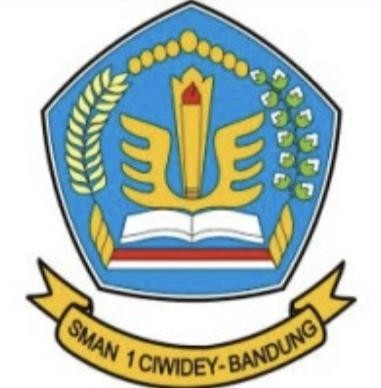
\includegraphics[width=0.3\linewidth]{images/sman1.png}
\end{figure}
%vertical space 2 cm
\vspace{2cm}

%nama penulis
\begin{center}
    Disusun Oleh: \\
    \begin{tabular}{ll}
         1.& Hasby Nauril Atoriq  \\
         2.& Abdan Fakih Makhlufi \\
         3.& Rezza Rahmadani \\
         4.& Riana Nur Rahmadina \\
         5.& Jihan Fathimatul Zahra\\
    \end{tabular}\\
    \vspace{0.5cm}
    Kelas X-1\\
    \vspace{1cm}
    \textbf{PEMERINTAH DAERAH PROVINSI JAWA BARAT}\\
    \textbf{DINAS PENDIDIKAN}\\
    \textbf{SMA NEGERI 1}\\
    \textbf{CIWIDEY}\\
    \textbf{2024}
\end{center}
\pagebreak

% \begin{center}
    \section*{LEMBAR PENGESAHAN KOORDINATOR}
    \addcontentsline{toc}{section}{\protect\numberline{}LEMBAR PENGESAHAN KOORDINATOR}
% \end{center}
\pagenumbering{Roman}
Laporan berjudul “Laporan projek penguatan profil pelajar pancasila gaya hidup berkelanjutan pengolahan sampah anorganik menjadi kerajinan geometri” telah diketahui dan disahkan. 
\vspace{2cm}
\\

\begin{table}[ht]
    \begin{tabular}{ll}
        Tanggal &: \\
        Oleh&: \\
    \end{tabular}
\end{table}
\vspace{5cm}
Koordinator Kelas P5\\
\newline

\vspace{5cm}
Junjun Junaedi, S.Pd.\\
\pagebreak

% \begin{center}
    \section*{KATA PENGANTAR}
    \addcontentsline{toc}{section}{\protect\numberline{}KATA PENGANTAR}
% \end{center}

Puji syukur kami panjatkan ke hadirat Tuhan Yang Maha Esa atas segala rahmat dan karunia-Nya sehingga kami dapat menyelesaikan laporan proyek “Penguatan Profil Pelajar Pancasila: Gaya Hidup Berkelanjutan Pengolahan Sampah Anorganik Menjadi Kerajinan Geometri” ini dengan baik. 

Laporan ini disusun sebagai salah satu bentuk implementasi dari program Penguatan Profil Pelajar Pancasila yang bertujuan untuk menanamkan nilai-nilai Pancasila dalam kehidupan sehari-hari, khususnya dalam hal gaya hidup berkelanjutan. Proyek ini berfokus pada pengolahan sampah anorganik menjadi kerajinan geometri, yang tidak hanya mengurangi dampak negatif sampah terhadap lingkungan, tetapi juga meningkatkan kreativitas dan keterampilan siswa. 

Kami menyadari bahwa laporan ini masih jauh dari sempurna. Oleh karena itu, kami sangat mengharapkan kritik dan saran yang membangun dari berbagai pihak demi perbaikan di masa mendatang. 

Area TeksAkhir kata, kami mengucapkan terima kasih kepada semua pihak yang telah membantu dalam penyusunan laporan ini, baik secara langsung maupun tidak langsung. Semoga laporan ini dapat bermanfaat dan memberikan inspirasi bagi pembaca\\

    \rightline{Pasirjambu, September 2024}
    \vspace{3cm}
    \rightline{Kelompok 1}
\pagebreak

% \begin{center}
    \section*{DAFTAR ISI}
    \addcontentsline{toc}{section}{\protect\numberline{}DAFTAR ISI}
% \end{center}
\renewcommand{\cftdot}{.}
\tableofcontents
\pagebreak
\begin{center}
    \section*{BAB I\\PENDAHULUAN}
    \addcontentsline{toc}{section}{\protect\numberline{}BAB I PENDAHULUAN}
\end{center}
\setcounter{section}{1}
\subsection{Latar Belakang}
\setcounter{page}{1}
\pagenumbering{arabic}
Dalam era modern ini, masalah lingkungan menjadi salah satu isu yang paling mendesak untuk diatasi. Salah satu masalah utama adalah meningkatnya jumlah sampah anorganik yang sulit terurai dan berdampak negatif terhadap lingkungan. Oleh karena itu, kami memilih subtema pengolahan sampah anorganik sebagai fokus utama proyek ini. Pengolahan sampah anorganik menjadi kerajinan geometri tidak hanya membantu mengurangi jumlah sampah yang mencemari lingkungan, tetapi juga memberikan nilai tambah melalui kreativitas dan inovasi. 

Pemilihan subtema ini didasarkan pada beberapa alasan. Pertama, sampah anorganik seperti plastik, kaca, dan logam memiliki waktu penguraian yang sangat lama, sehingga pengelolaannya memerlukan perhatian khusus. Kedua, dengan mengolah sampah anorganik menjadi produk kerajinan, kami dapat memberikan contoh konkret bagaimana sampah dapat diubah menjadi sesuatu yang bermanfaat dan bernilai ekonomi. Ketiga, proyek ini juga bertujuan untuk meningkatkan kesadaran masyarakat, khususnya para pelajar, tentang pentingnya menjaga lingkungan melalui tindakan nyata. 

Produk kerajinan geometri dipilih karena memiliki daya tarik estetika dan fungsional yang tinggi. Bentuk-bentuk geometris yang dihasilkan dari pengolahan sampah anorganik dapat digunakan sebagai dekorasi, alat peraga pendidikan, atau bahkan barang-barang fungsional sehari-hari. Dengan demikian, proyek ini tidak hanya berkontribusi pada pengurangan sampah, tetapi juga mendorong kreativitas dan keterampilan siswa dalam menciptakan produk yang inovatif dan ramah lingkungan \cite{GeometriArt},

\subsection{Tujuan}
Proyek ini dilaksanakan dengan beberapa tujuan utama sebagai berikut:  
\begin{enumerate}
    \item     Mengurangi Dampak Lingkungan: Mengolah sampah anorganik menjadi kerajinan geometri bertujuan untuk mengurangi jumlah sampah yang mencemari lingkungan. Dengan demikian, proyek ini berkontribusi pada upaya pelestarian lingkungan dan pengurangan polusi. 
    \item Meningkatkan Kreativitas dan Keterampilan: Melalui kegiatan ini, siswa diharapkan dapat mengembangkan kreativitas dan keterampilan mereka dalam mengolah bahan-bahan yang tidak terpakai menjadi produk yang bernilai. Proyek ini juga mendorong inovasi dalam menciptakan barang-barang yang estetis dan fungsional. 
    \item     Memberikan Nilai Ekonomi: Produk kerajinan yang dihasilkan dari proyek ini memiliki potensi untuk dijual, sehingga dapat memberikan nilai ekonomi tambahan. Hal ini juga mengajarkan siswa tentang konsep ekonomi sirkular dan bagaimana mengubah limbah menjadi sumber daya yang bermanfaat. 
\end{enumerate}

\subsection{Manfaat}
Proyek pengolahan sampah anorganik menjadi kerajinan geometri ini memberikan berbagai manfaat yang signifikan, baik bagi lingkungan, siswa, maupun masyarakat secara umum. Manfaat-manfaat tersebut antara lain: 
\begin{enumerate}
    \item     Manfaat Lingkungan: Proyek ini membantu mengurangi jumlah sampah anorganik yang mencemari lingkungan. Dengan mengolah sampah menjadi produk yang berguna, proyek ini berkontribusi pada pengurangan polusi dan pelestarian lingkungan. 
    \item     Manfaat Pendidikan: Melalui kegiatan ini, siswa mendapatkan kesempatan untuk belajar tentang pentingnya pengelolaan sampah dan konsep daur ulang. Mereka juga mengembangkan keterampilan praktis dalam mengolah bahan-bahan bekas menjadi produk yang bernilai, serta meningkatkan kreativitas dan inovasi. 
\end{enumerate}

\subsection{Ruang Lingkup (Sasaran}
Proyek pengolahan sampah anorganik menjadi kerajinan geometri ini memiliki sasaran yang jelas dan terarah, meliputi: 
\begin{enumerate}
    \item     Siswa Sekolah: Sasaran utama dari kegiatan ini adalah siswa sekolah, khususnya mereka yang terlibat langsung dalam proses pengolahan sampah dan pembuatan kerajinan. Melalui proyek ini, siswa diharapkan dapat meningkatkan kesadaran lingkungan, kreativitas, dan keterampilan praktis mereka. 
    \item     Guru dan Tenaga Pendidik: Guru dan tenaga pendidik juga menjadi sasaran penting dalam proyek ini. Mereka berperan sebagai fasilitator dan pembimbing bagi siswa, serta membantu dalam mengintegrasikan konsep pengelolaan sampah dan daur ulang ke dalam kurikulum pendidikan. 
    \item     Masyarakat Sekitar: Proyek ini juga menyasar masyarakat sekitar sekolah. Dengan melibatkan masyarakat dalam kegiatan kampanye dan pameran hasil kerajinan, diharapkan dapat meningkatkan kesadaran dan partisipasi aktif mereka dalam upaya pengelolaan sampah dan pelestarian lingkungan. 
\end{enumerate}
\pagebreak
% \begin{center}
    \section*{BAB II\\PELAKSANAAN KEGIATAN}
    \addcontentsline{toc}{section}{\protect\numberline{}BAB II PELAKSANAAN KEGIATAN}
% \end{center}
\setcounter{section}{2}
 \setcounter{subsection}{0}
\subsection{Waktu dan Tempat Kegiatan}

 \begin{table}[ht]
     \centering
     \begin{tabular}{lll}
          1. Waktu&:  &27 Agustus -- 17 September 2024 \\
          2. Tempat Kegiatan&:  & SMAN 1 Ciwidey \\
     \end{tabular}
 \end{table}

 \subsection{Jadwal Kegiatan}
 \begin{table}[ht]
     \centering
     \begin{tabular}{|c|c|c|}
     \hline
     \rowcolor[HTML]{9B9B9B}
         No. & Hari, Tanggal  & Kegiatan \\ \hline
         1 & Rabu, 27 Agustus 2024  & Persiapan Pembelian Alat dan Bahan \\ \hline
         2 & Rabu, 28 Agustus 2024 & Pembelian Alat dan Bahan \\ \hline
         3 & Rabu, 11 September 2024 & Pembuatan Laporan\\ \hline
         4 & Minggu, 15 September 2024 & Revisi dan Penyelesaian Laporan\\ \hline
     \end{tabular}
 \end{table}
 \subsection{Alat dan Bahan}
 \begin{enumerate}
     \item Gunting
     \item Lem
     \item Stik Eskrim
     \item Kerta A4
 \end{enumerate}
 \subsection{Langkah Langkah Pembuatan Produk}
 \subsubsection{Tahap Persiapan}
 
 \begin{table}[ht]
     \centering
     \begin{tabular}{|c|c|c|}
     \hline
     \rowcolor[HTML]{9B9B9B}
         No. & Hari, Tanggal  & Hasil Diskusi Tahap Persiapan \\ \hline
         1 & Rabu, 27 Agustus 2024  & Persiapan Pembelian Alat dan Bahan \\ \hline
         2 & Rabu, 27 Agustus 2024 & Pembelian Alat dan Bahan \\ \hline
         3 & Rabu, 27 Agustus 2024 & Penentuan Tema\\ \hline
         4 & Kamis, 28 Agustus 2024 & Pengumpulan Projek\\ \hline
     \end{tabular}
 \end{table}
 \subsubsection{Tahap Pelaksanaan}
 \begin{table}[ht]
     \centering
     \begin{tabular}{|c|c|c|c|}
     \hline
     \rowcolor[HTML]{9B9B9B}
     No. & Hari, Tanggal  & Kegiatan Tahap Pelaksanaan & Dokumentasi\\ \hline
     1 & Kamis, 28 Agustus 2024  & Pembuatan Sketsa & Gambar 1\\ \hline
     2 & Kamis, 28 Agustus 2024 & Pengukuran Bahan & Gambar 2\\ \hline
     3 & Kamis, 28 Agustus 2024 & Pengeleman Bahan & Gambar 3\\ \hline
     4 & Kamis, 28 Agustus 2024 & Penempelan Bahan & Gambar 4\\ \hline
     \end{tabular}
 \end{table}
\subsubsection{Tahap Penyusunan Laporan}
 \begin{table}[ht]
     \centering
     \begin{tabular}{|c|c|c|}
     \hline
     \rowcolor[HTML]{9B9B9B}
     No. & Hari, Tanggal  & Perkembangan Laporan\\ \hline
     1 & Rabu, 11 September 2024  & Penyusunan Laporan\\ \hline
     2 & Rabu, 11 September 2024 & Penyusunanan Kata pengantar dan BAB I\\ \hline
     3 & Rabu, 11 September 2024 & Penyusunan BAB II\\ \hline
     4 & Minggu, 15 September 2024 & Revisi dan penambahan informasi\\ \hline
     \end{tabular}
 \end{table}
 \pagebreak
    \section*{BAB III\\KESIMPULAN DAN SARAN}
    \addcontentsline{toc}{section}{\protect\numberline{}BAB III KESIMPULAN DAN SARAN}
\setcounter{section}{3}
 \setcounter{subsection}{0}
\subsection{Kesimpulan}
Proyek “Penguatan Profil Pelajar Pancasila: Gaya Hidup Berkelanjutan Pengolahan Sampah Anorganik Menjadi Kerajinan Geometri” telah berhasil dilaksanakan dengan baik. Melalui proyek ini, siswa tidak hanya belajar tentang pentingnya pengelolaan sampah dan daur ulang, tetapi juga mengembangkan kreativitas dan keterampilan mereka dalam mengolah sampah anorganik menjadi produk yang bernilai. Proyek ini juga berhasil meningkatkan kesadaran lingkungan di kalangan siswa dan masyarakat sekitar, serta memberikan contoh konkret bagaimana sampah dapat diubah menjadi sumber daya yang bermanfaat. 

Secara keseluruhan, proyek ini memberikan manfaat yang signifikan bagi lingkungan, pendidikan, ekonomi, dan sosial. Dengan mengurangi jumlah sampah anorganik yang mencemari lingkungan, meningkatkan keterampilan dan kreativitas siswa, serta memberikan nilai ekonomi tambahan melalui produk kerajinan, proyek ini telah mencapai tujuan-tujuan yang telah ditetapkan. 
\subsection{Saran}
\begin{enumerate}
  \item     Pengembangan Proyek: Untuk keberlanjutan proyek ini, disarankan agar kegiatan pengolahan sampah anorganik menjadi kerajinan geometri terus dikembangkan dan diperluas. Melibatkan lebih banyak siswa dan masyarakat dalam kegiatan ini akan meningkatkan dampak positifnya. 
  \item     Kerjasama dengan Pihak Lain: Disarankan untuk menjalin kerjasama dengan pemerintah daerah, lembaga pendidikan, dan organisasi lingkungan untuk mendapatkan dukungan dan sumber daya yang lebih besar. Kerjasama ini juga dapat membantu dalam memperluas jangkauan proyek ke wilayah yang lebih luas. 
  \item     Peningkatan Edukasi: Edukasi tentang pengelolaan sampah dan daur ulang perlu ditingkatkan, baik di dalam kurikulum sekolah maupun melalui kegiatan ekstrakurikuler. Dengan demikian, kesadaran dan partisipasi siswa dalam menjaga lingkungan akan semakin meningkat. 
  \item     Pemasaran Produk: Produk kerajinan yang dihasilkan dari proyek ini memiliki potensi untuk dijual. Disarankan untuk mengembangkan strategi pemasaran yang efektif agar produk-produk ini dapat dikenal dan diminati oleh masyarakat luas, sehingga memberikan nilai ekonomi tambahan. 
  \item     Evaluasi dan Perbaikan: Melakukan evaluasi secara berkala terhadap pelaksanaan proyek ini sangat penting untuk mengetahui kekurangan dan mencari solusi perbaikan. Dengan demikian, proyek ini dapat terus berkembang dan memberikan manfaat yang lebih besar di masa mendatang\cite{GeometriArt},
\pagebreak
\end{enumerate}
    \section*{DAFTAR PUSTAKA}
    \addcontentsline{toc}{section}{\protect\numberline{}DAFTAR PUSTAKA}
    \medskip
    \printbibliography
\pagebreak
    \section*{LAMPIRAN}
    \addcontentsline{toc}{section}{\protect\numberline{}LAMPIRAN}
    \begin{figure}[ht]
      \begin{center}
        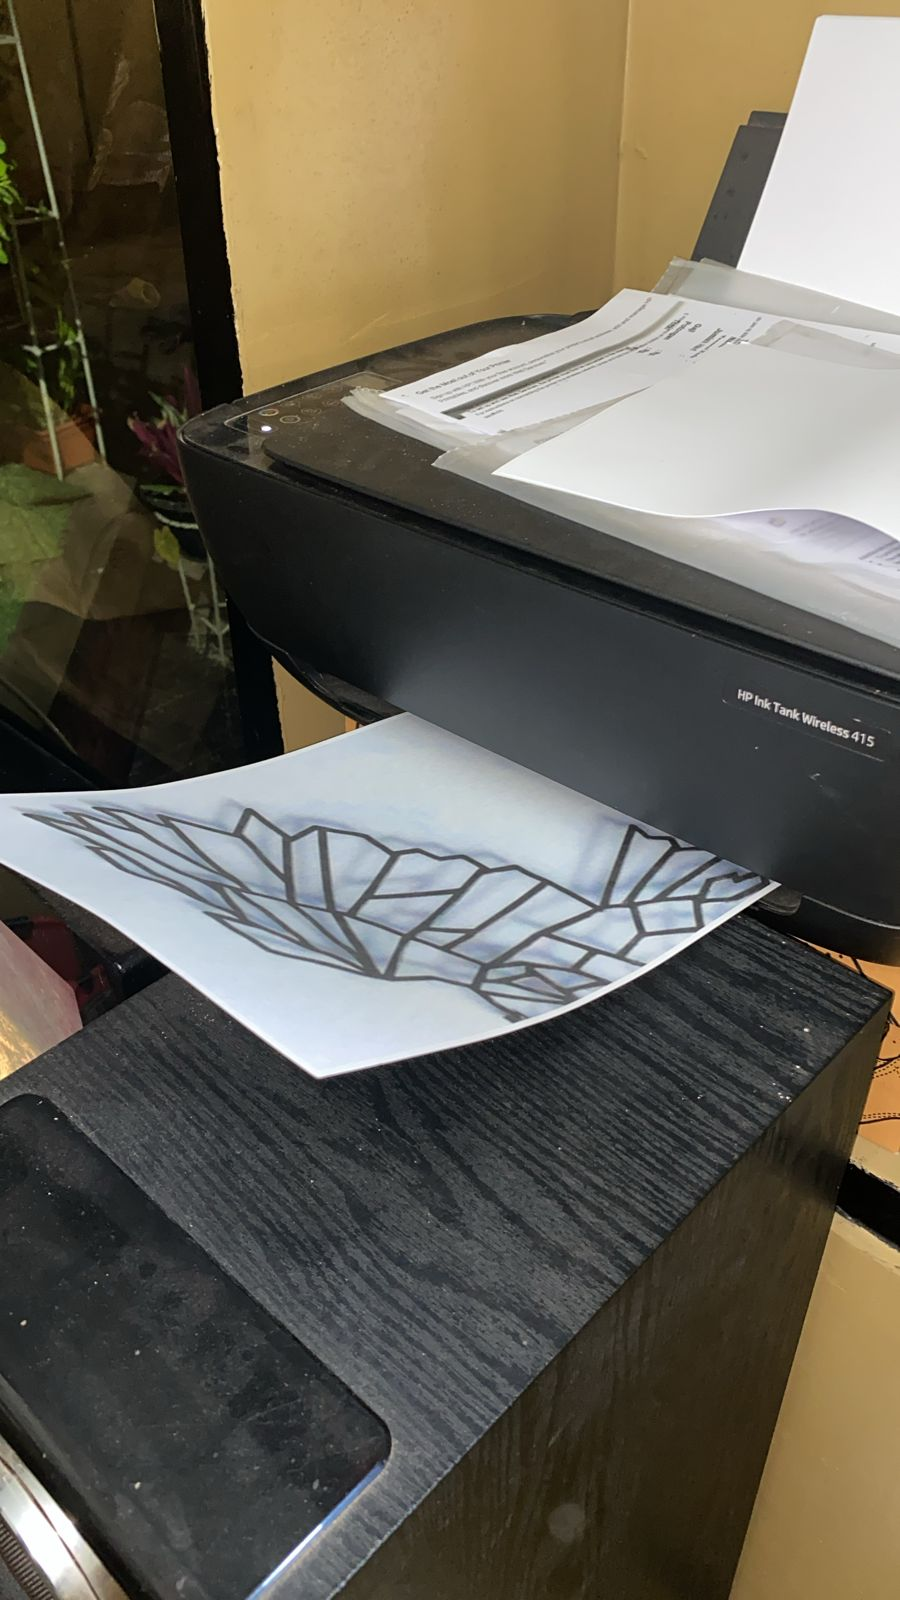
\includegraphics[width=0.50\textwidth]{images/gambar1.jpeg}
      \end{center}
      \caption{Pencetakan Sketsa}\label{fig:}
    \end{figure}
   \begin{figure}
    \begin{center}
      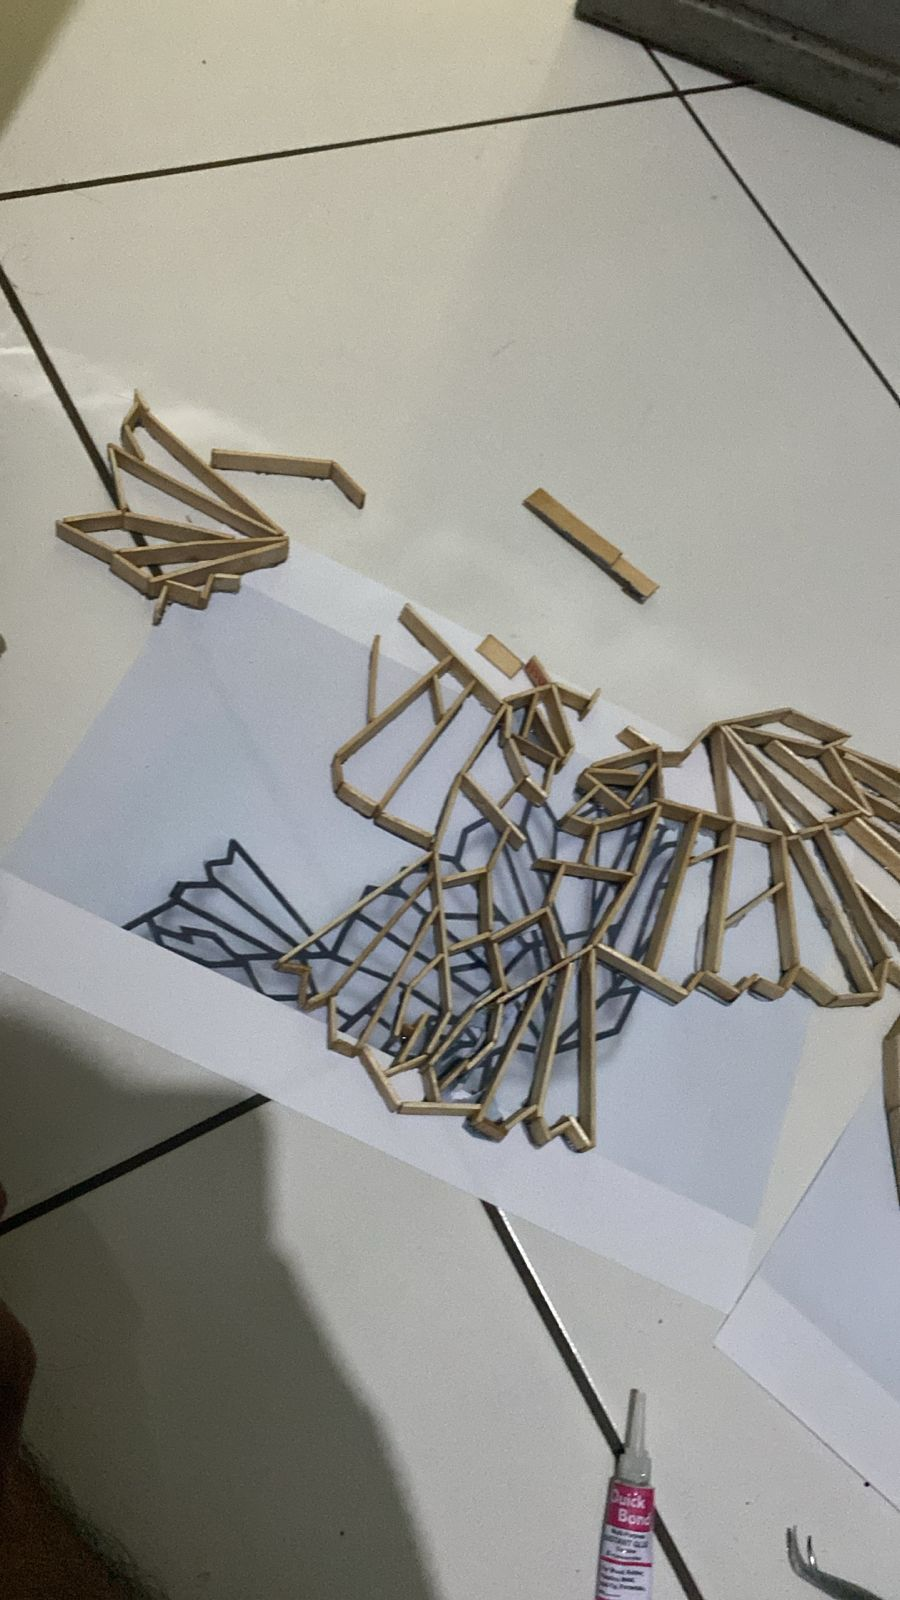
\includegraphics[width=0.50\textwidth]{images/gambar2.jpeg}
    \end{center}
    \caption{Pengukuran Bahan}\label{fig:}
   \end{figure}
   \begin{figure}
    \begin{center}
      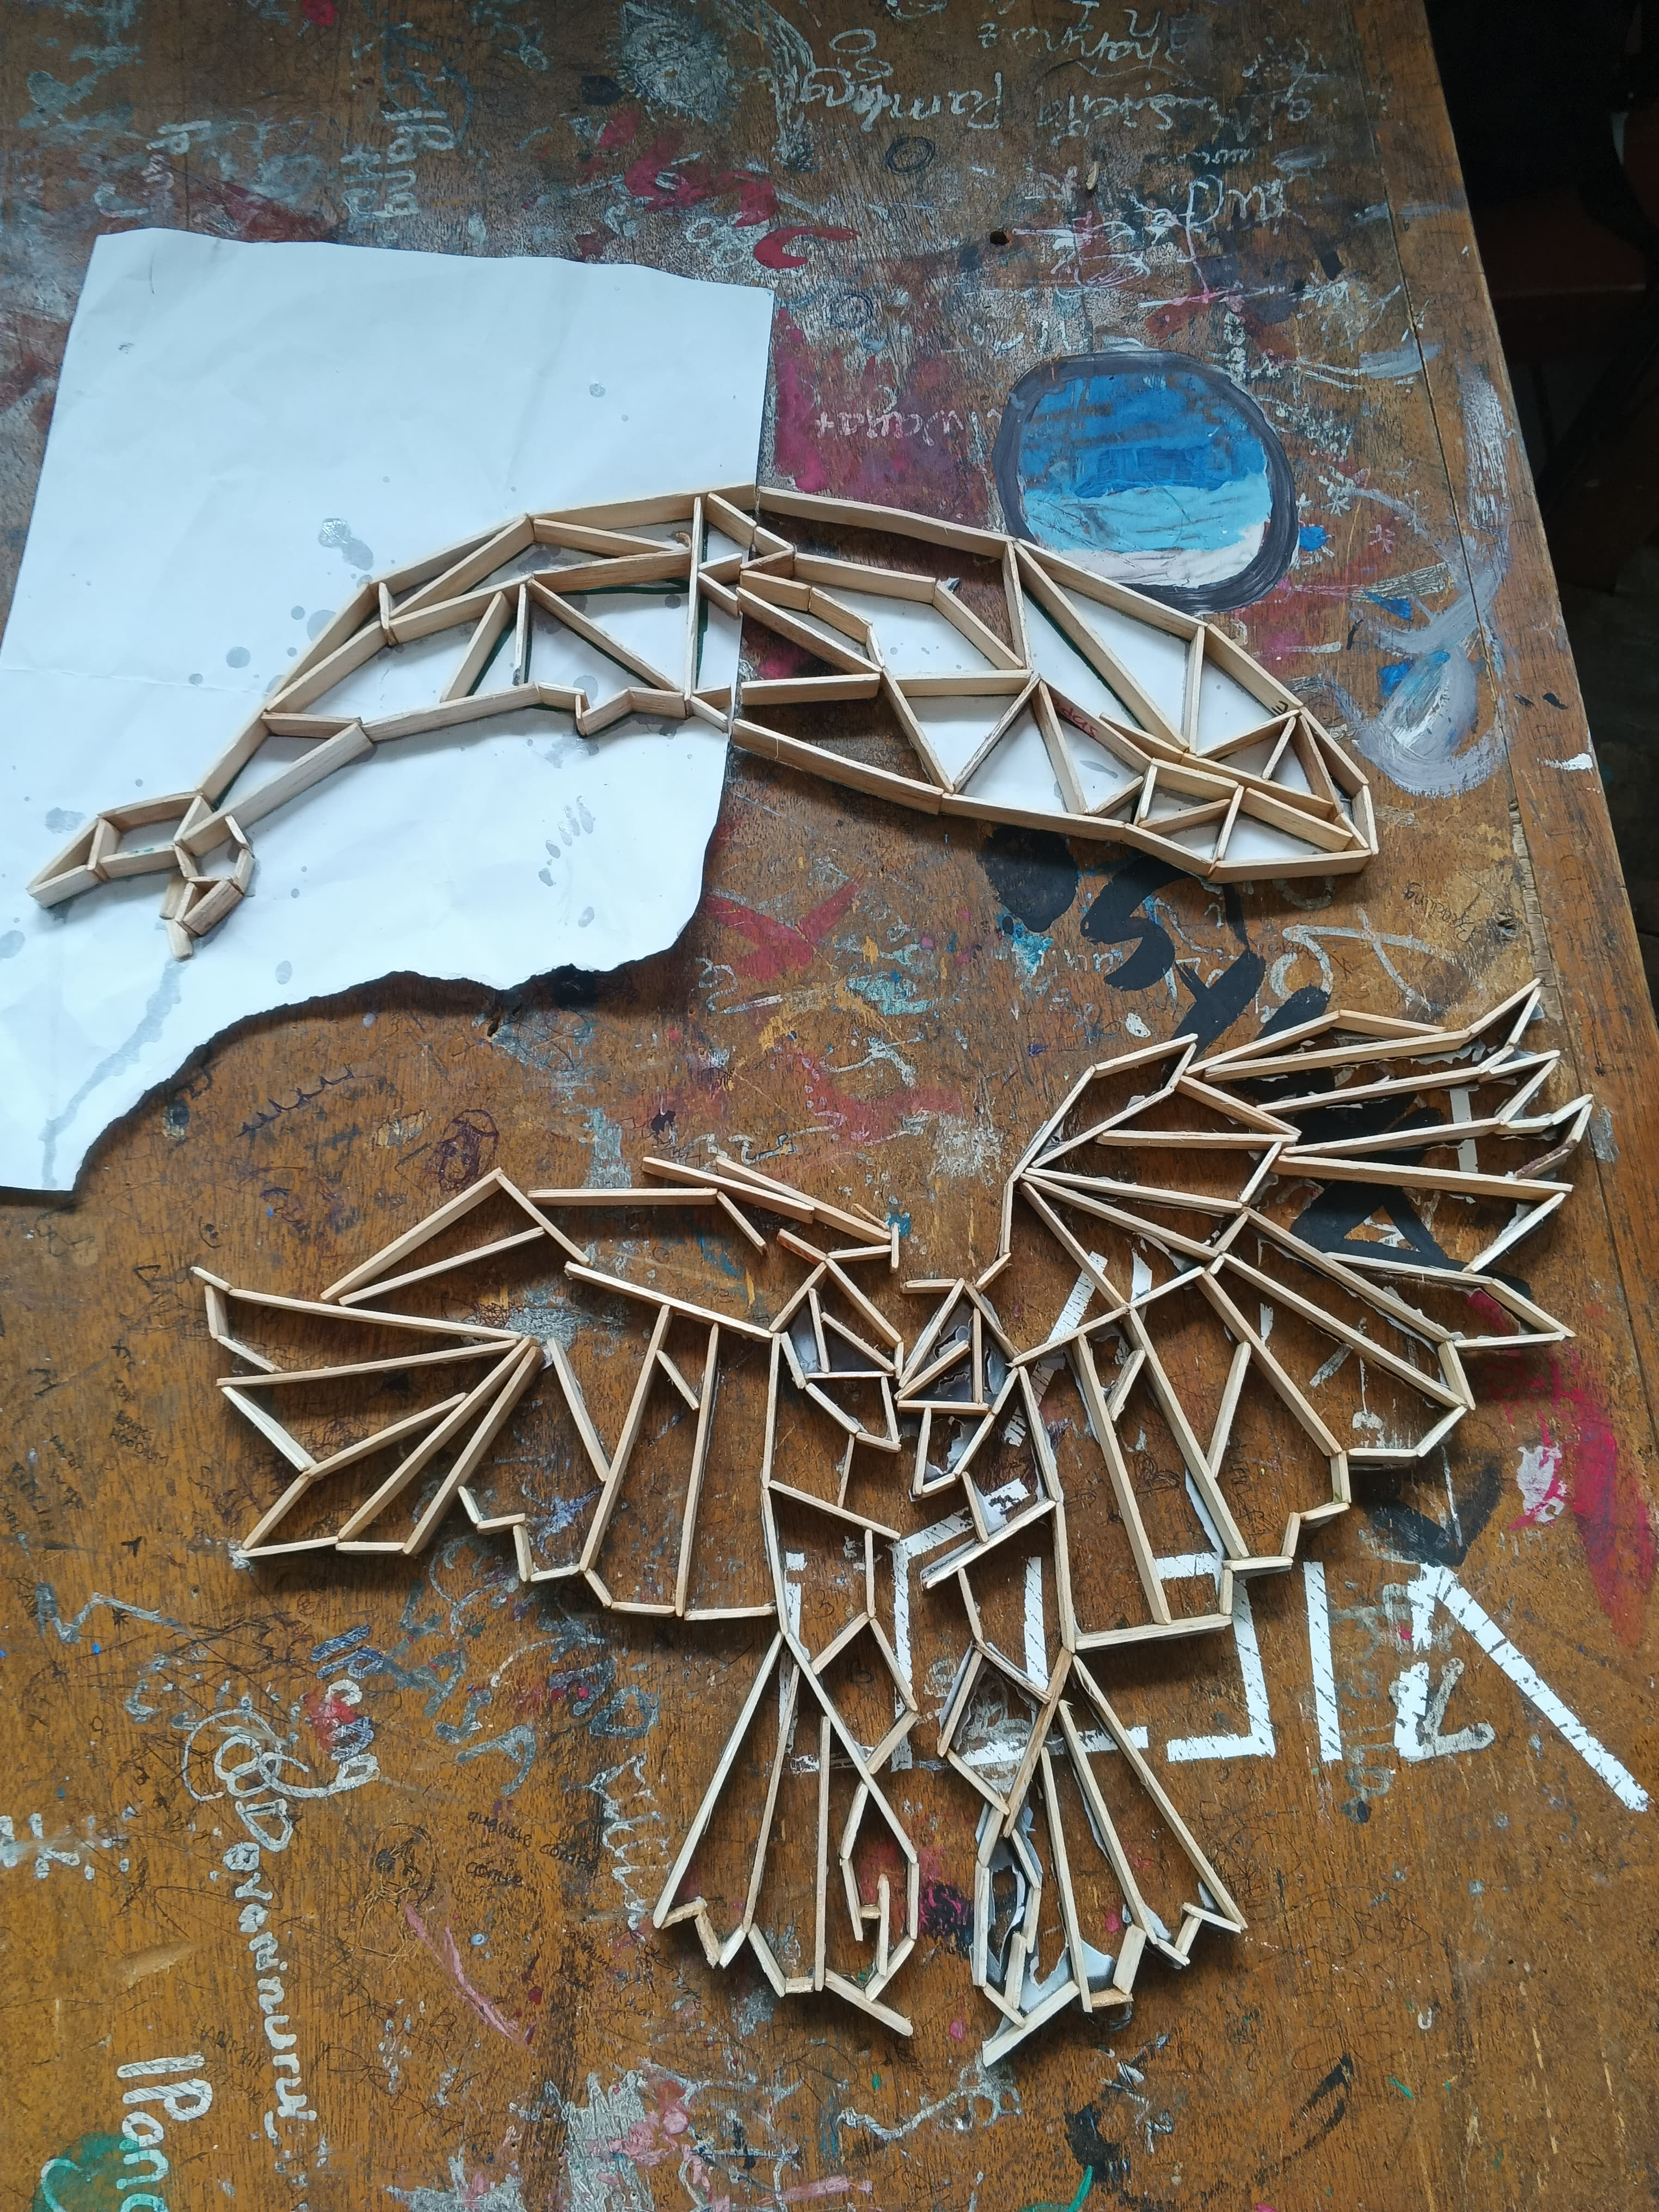
\includegraphics[width=0.50\textwidth]{images/gambar3.jpeg}
    \end{center}
    \caption{Pengeleman Bahan}\label{fig:}
   \end{figure}
   \begin{figure}
    \begin{center}
      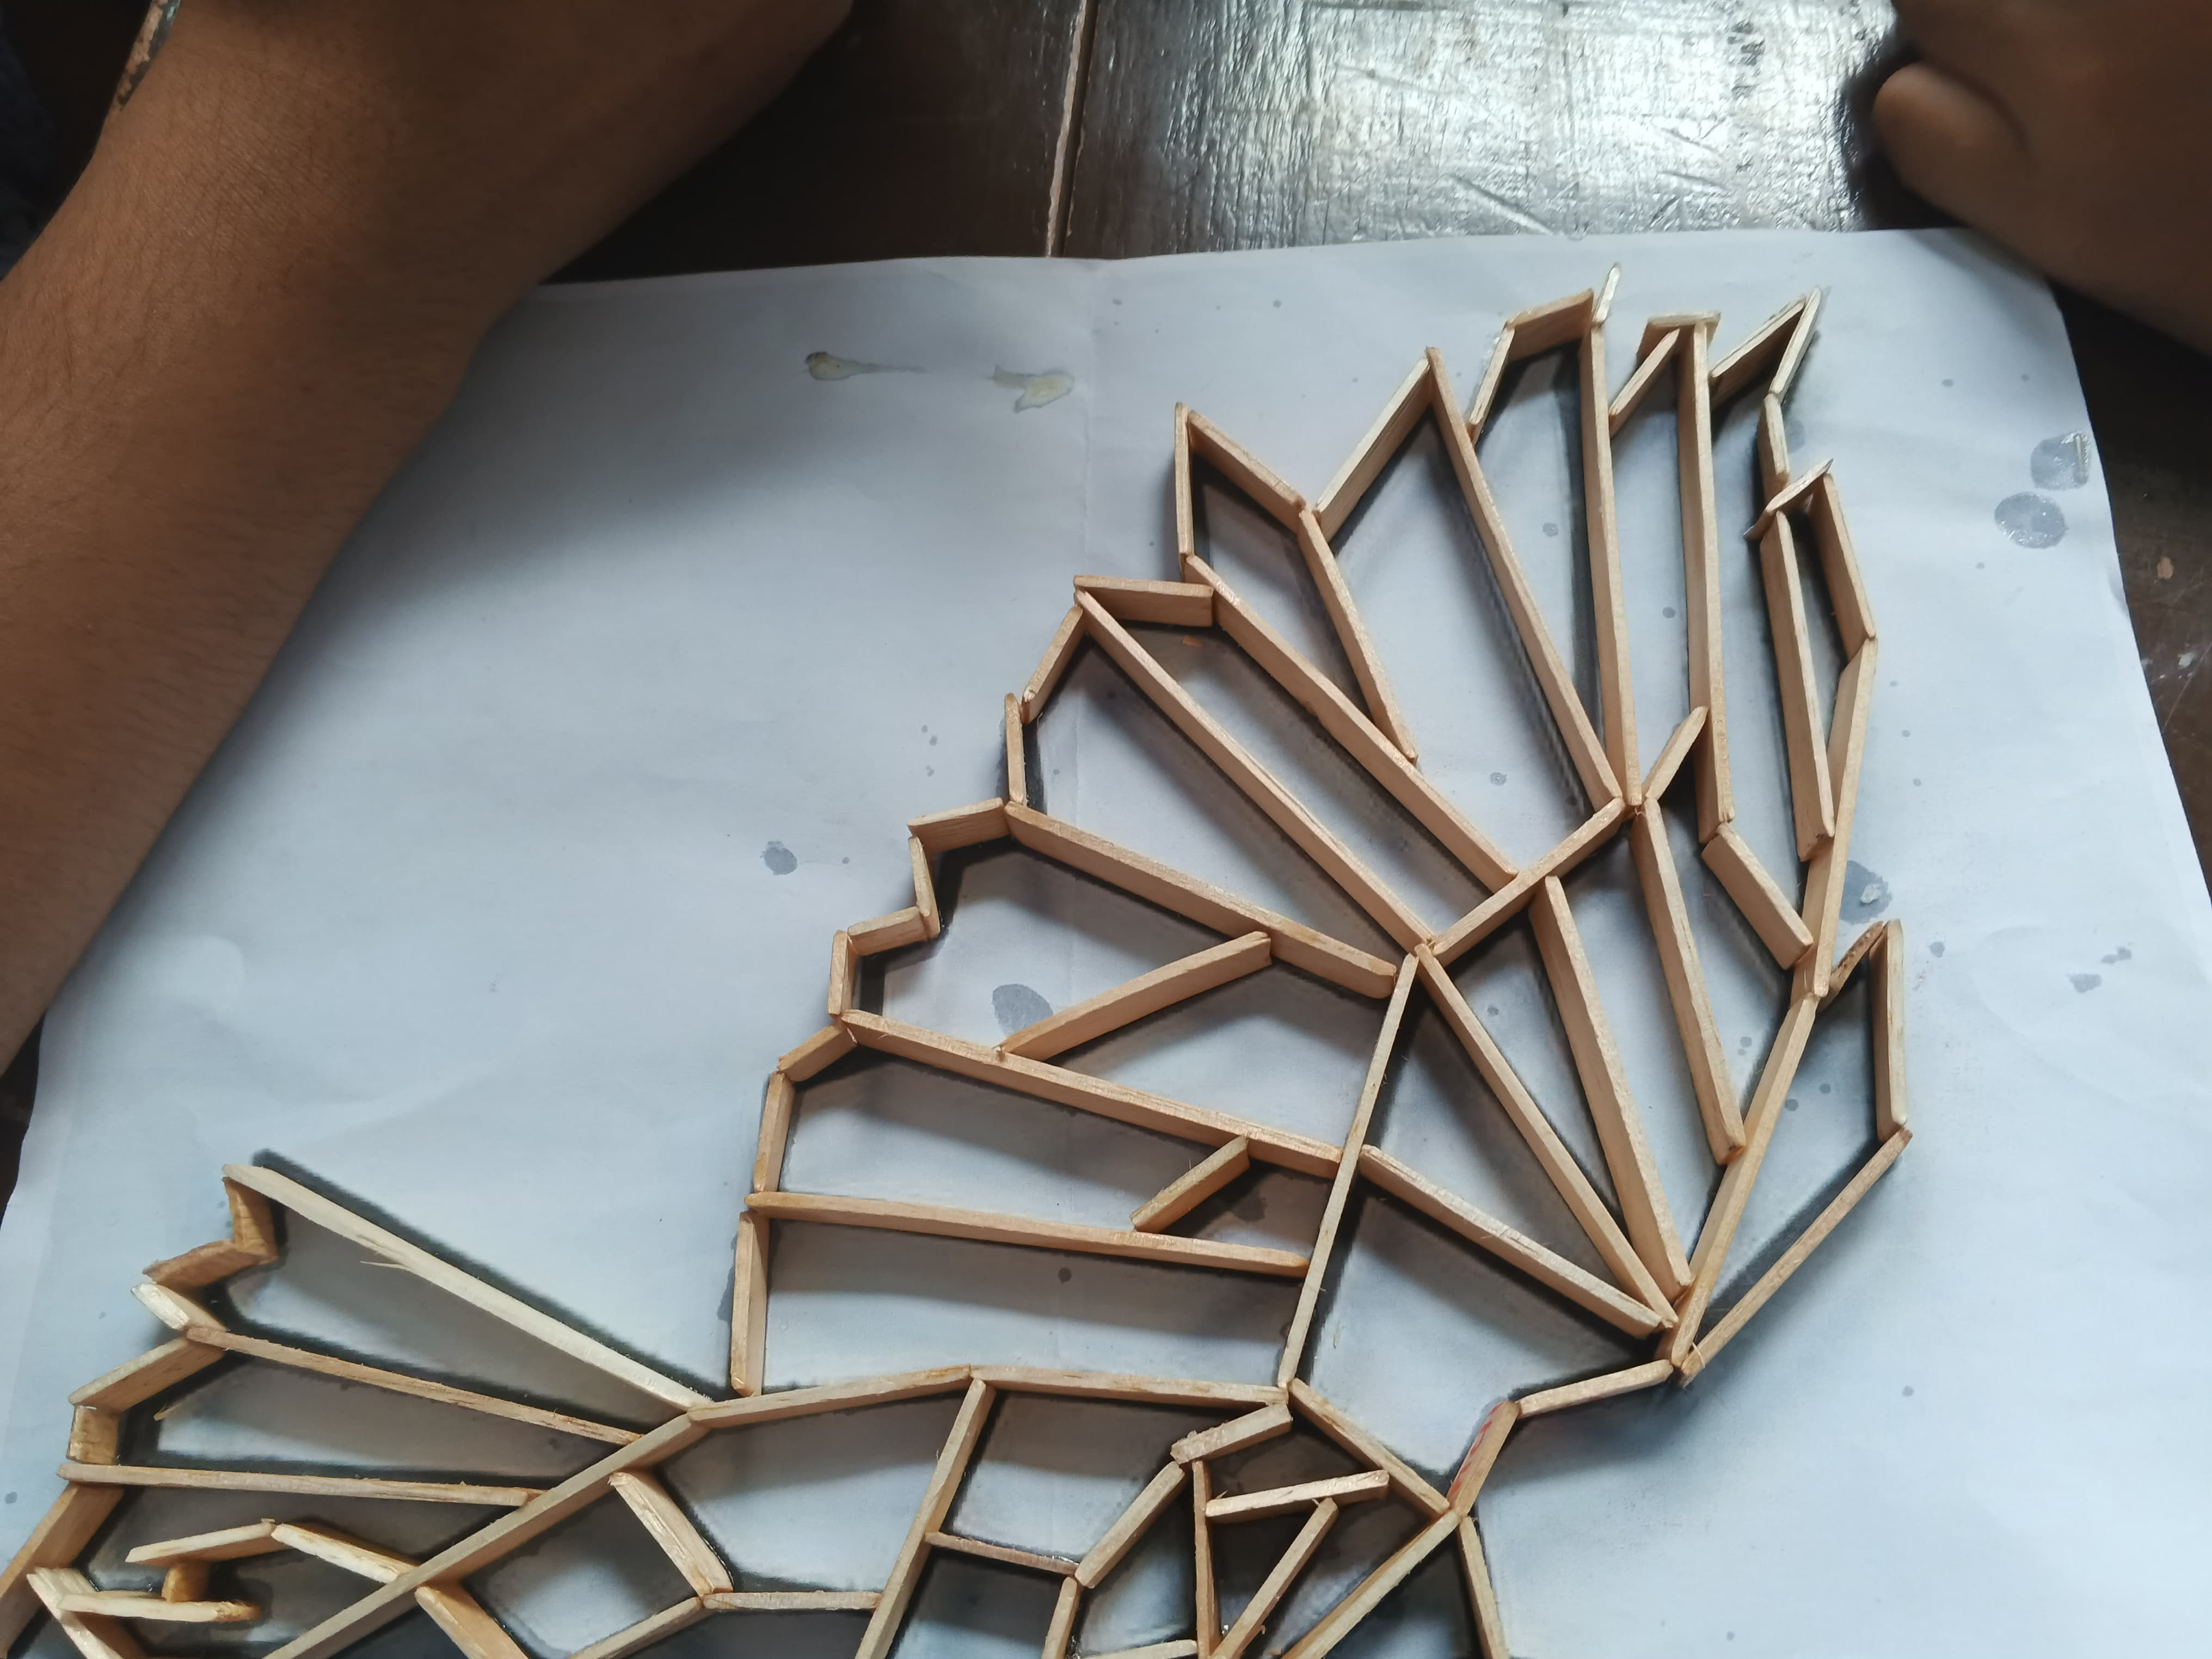
\includegraphics[width=0.50\textwidth]{images/gambar4.jpeg}
    \end{center}
    \caption{Penempelan Bahan di Sketsa}\label{fig:}
   \end{figure}
    
\end{document}
